% ****** Start of file aipsamp.tex ******
%
%   This file is part of the AIP files in the AIP distribution for REVTeX 4.
%   Version 4.1 of REVTeX, October 2009
%
%   Copyright (c) 2009 American Institute of Physics.

% Use this file as a source of example code for your aip document.
% Use the file aiptemplate.tex as a template for your document.
\documentclass[%
	aip,
	jmp,%
	amsmath,amssymb,
	%preprint,%
	reprint,%
	%author-year,%
	%author-numerical,%
]{revtex4-1}
%\extrafloats{1000}
\usepackage{morefloats}% Include figure files
\usepackage{graphicx}% Include figure files
\usepackage{grffile}
\usepackage{afterpage}
\usepackage{dcolumn}% Align table columns on decimal point
\usepackage{bm}% bold math
%\usepackage[mathlines]{lineno}% Enable numbering of text and display math
%\linenumbers\relax % Commence numbering lines
\usepackage{multirow}
\usepackage{color} % for the notes
\usepackage{etex}
\reserveinserts{58}
%\usepackage{morefloats}
\usepackage{hyperref}
\usepackage{xcolor}
\usepackage{amsmath}
\hypersetup{
	colorlinks,
	linkcolor={red!50!black},
	citecolor={blue!50!black},
	urlcolor={blue!80!black}
}

\usepackage{xr}
\externaldocument{supportingInformation}
\maxdeadcycles=1000

\usepackage{placeins}
\begin{document}

\preprint{XXXXX (preprint)}

%\title[Evolution of interaction networks]{On the evolution of interaction networks: primitive typology of vertex, prominence of measures and activity statistics}% Force line breaks with \\
%\title[Evolution of interaction networks]{On the evolution of interaction networks: a primitive typology of vertex}% Force line breaks with \\
%\title[Stability of interaction networks]{Stability in human interaction networks: sector relative sizes, prominence of topological measures and time activity statistics.}% Force line breaks with \\
%\title[Stability in human interaction networks]{Sector relative sizes and topological metrics time stability in human interaction networks}% Force line breaks with \\
\title[Distances between histograms]{A distance metric between histograms
through the the Kolmogorov-Smirnov test statistic: specification, measures reference and example uses}% Force line breaks with \\
\author{Renato Fabbri}%
\homepage{http://ifsc.usp.br/~fabbri/}
\email{fabbri@usp.br}
\affiliation{ 
	S\~ao Carlos Institute of Physics, University of S\~ao Paulo (IFSC/USP),
	PO Box 369, 13560-970, S\~ao Carlos, SP, Brazil %\\This line break forced with \textbackslash\textbackslash
}

\date{\today}% It is always \today, today,
%  but any date may be explicitly specified

\begin{abstract}
This document presents reference values for a distance metric
derived from the Kolmogorov-Smirnov test statistic $D_{n,n'}$.
Each measure of $D_{n,n'}$ is a distance between two histograms,
which is normalized by the number of observations in each sample
to yield p-values $c'$, i.e. values for which 
higher levels of significance $\alpha>c'$ implies the rejection of the null hypothesis.
Benchmarks for the implementation are delivered by comparing samples from known distributions.
Pattern examples in real data enables further
insight in the robustness and power of $c'$.
\end{abstract}

\pacs{05.10-a,}% PACS, the Physics and Astronomy
\keywords{Kolmogorov-Smirnov test, statistic, benchmark, distance measure, histogram}
\maketitle
\section{Introduction}\label{sec:intro}

% $D_{n,n'}$
%depicted in Figure~\ref{fig:kolms}


Be $F$ and $F'$ two empirical cumulative distributions,
where $n$ and $n'$ are the number of observations on each sample.
The two-sample Kolmogorov-Smirnov test rejects the null hypothesis
that the histograms are the outcome of the same underlying distribution
if:
\begin{equation}\label{eq:ks}
D_{F,F'} > c(\alpha)\sqrt{\frac{n+n'}{nn'}}
\end{equation}

\noindent where $D_{F,F'}=sup_x[F-F']$ as in Figure~\ref{fig:dnn}
and $c(\alpha)$ is related to the level of significance $\alpha$ by:

\begin{table}[h!]
\centering
\begin{tabular}{|l||c|c|c|c|c|c|}\hline
$\alpha$    & 0.1  & 0.05 & 0.025 & 0.01 & 0.005 & 0.001 \\\hline
$c(\alpha)$ & 1.22 & 1.36 & 1.48  & 1.63 & 1.73  & 1.95  \\\hline
\end{tabular}
\end{table}

If distributions are drawn from empirical data, $D_{F,F'}$ is given as are $n$ and $n'$.
All terms in equation~\ref{eq:ks} are positive and $c(\alpha)$ can be isolated:

\begin{equation}\label{eq:ks2}
	c(\alpha) < \frac{D_{n,n'}}{\sqrt{\frac{n+n'}{nn'}}} = c
\end{equation}

%Tables~\ref{tab:kolSub}-\ref{tab:kolPctInter} are populated with values for $c'(\alpha)$
When $c$ is high, low values of $\alpha$ favor rejecting the null hypothesis.
In fact, $c$ can be normalized to yield p-values.

\begin{figure}[!h]
	\centering
	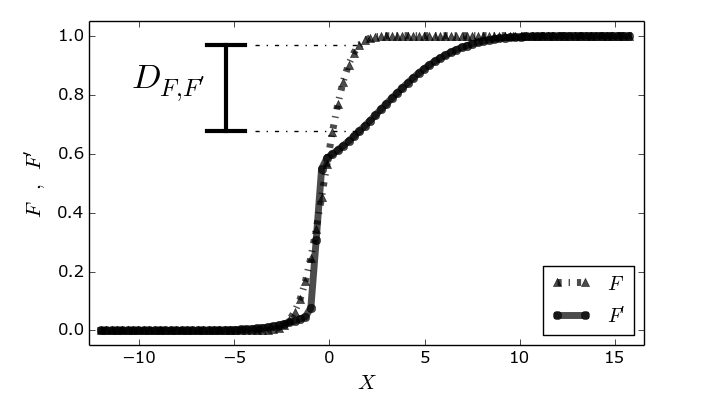
\includegraphics[width=0.44\textwidth]{figs/Dnn}
	\caption{The Kolmogorov-Smirnov statistic $D_{F,F'}$: the maximum difference between
		two cumulative distribution functions.}
	\label{fig:dnn}
\end{figure}

Hight values of $c$ favor rejecting the null hypothesis.
For example, if the significance level is $\alpha=0.01$,
then $c$ greater than $1.7$
implies the rejection of the null hypothesis and
suggests that $F$ and $F'$
are outcomes of different distributions.
Of core importance in this study is to regard the $c$ statistic
as a measure of distance between both distributions~\cite{kolm}.
The main contribution of the following sections is the
explicit display of reference values of $c$
from which one might derive knowledge from
$c$ measures or even from a single value of $c$.

\subsection{Philosophical and technological note}
Difference and equivalence is of central role in human cognition,
philosophy and science.
This fact is so deeply recognized that thinkers often reduce
thought to classifications, e.g. through the
mathematical concept of equivalence classes~\cite{deleuze}.
Histograms are very immediate and informative
roughly wherever there is a phenomenon of interest which can yield measurements.
This present document should enable conclusions to be drawn about 
the equivalence (and difference)
of the processes underlying sets of measurements for a very
broad range of phenomena.
The following tables 
validate the mathematical framework
and the software implementation.

\subsection{Document outline}
Section~\ref{sec:simulations} exposes reference values drawn from simulations.
Section~\ref{sec:empirical} exemplifies the use of such reference values
to make sense of phenomena.
Section~\ref{sec:conc} holds final remarks.
Software and data specification are given in Appendix~\ref{ap:soft}.

\section{References through simulations}\label{sec:simulations}
On every case, values of $c$ are given for simulations involving
at least normal, uniform, Weibull and power function distributions.
The rendering of this article is automated to ease changes in
the settings with which the results are reported.
\input{aux/preambule1}

\subsection{When the null hypothesis is true}
If the null hypothesis is true, than the number
of rejections of the null hypothesis (that is: $c>c(\alpha)$)
in $N_c$ comparisons should not exceed $\alpha N_c$.
To verify this, let $C=\{c_i\}$ be a set of $c$ measures,
and $C(\alpha)=\{c : c>c(\alpha)\}$.
Be $|C(\alpha)|$ the cardinality of $C(\alpha)$,
i.e. the number of comparisons in which the two-sample Kolmogorov-Smirnov
test rejects the null hypothesis for a given $\alpha$.
This section reports that
$|C(\alpha)|$ very rarely exceeds $\alpha N_c$,
for all probability distributions and settings.
Also important are that
$c>c(\alpha)$ in many cases
and that the tabulated $\alpha$ values
are also good estimates of the upper limit
of the frequency of such an event.

%\begin{itemize}
%	\item $c'>c(\alpha)$ in many cases, and $\alpha N_c$ is a good upper limit to keep in mind.
%	\item 
%\end{itemize}

% Input tables
% any plot? If std is ~stable, plots of the mean of c~(\alpha) are compact and informative
\begin{table}[h!]
\begin{center}
\begin{tabular}{| l | c | c | c | c | c |}\hline
$\alpha N_c$ & $\alpha$ & $c(\alpha)$ & $|C_1(\alpha)|$ & $|C_2(\alpha)|$ & $|C_3(\alpha)|$ \\\hline
10.0 & 0.100 & 1.22 & 8 & 7 & 5 \\\hline
5.0 & 0.050 & 1.36 & 1 & 2 & 2 \\\hline
2.5 & 0.025 & 1.48 & 1 & 0 & 1 \\\hline
1.0 & 0.010 & 1.63 & 1 & 0 & 0 \\\hline
0.5 & 0.005 & 1.73 & 1 & 0 & 0 \\\hline
0.1 & 0.001 & 1.95 & 0 & 0 & 0 \\\hline
\end{tabular}
\caption{The theoretical maximum number $\alpha N_c$ of rejections
        of the null hypothesis for significance levels $\alpha$.
        The $c_1$ values were calculated using simulations of normal distributions with $\mu=0$ and $\sigma=1$.
        The $c_2$ values were calculated using simulations of normal distributions with $\mu=3$ and $\sigma=2$.
        The $c_3$ values were calculated using simulations of normal distributions with $\mu=6$ and $\sigma=3$.
        Over all $N_c$ comparisons,
         $\mu(c_1)=0.7775$ and $\sigma(c_1)=0.2573$,
         $\mu(c_2)=0.7976$ and $\sigma(c_2)=0.2388$,
         $\mu(c_3)=0.7596$ and $\sigma(c_3)=0.2292$ .
        }
\end{center}
\end{table}
\begin{table}[h!]
\begin{center}
\begin{tabular}{| l | c | c | c | c | c |}\hline
$\alpha N_c$ & $\alpha$ & $c(\alpha)$ & $|C_1(\alpha)|$ & $|C_2(\alpha)|$ & $|C_3(\alpha)|$ \\\hline
100.0 & 0.100 & 1.22 & 93 & 88 & 95 \\\hline
50.0 & 0.050 & 1.36 & 43 & 42 & 39 \\\hline
25.0 & 0.025 & 1.48 & 19 & 28 & 17 \\\hline
10.0 & 0.010 & 1.63 & 7 & 10 & 12 \\\hline
5.0 & 0.005 & 1.73 & 4 & 4 & 8 \\\hline
1.0 & 0.001 & 1.95 & 1 & 0 & 1 \\\hline
\end{tabular}
\caption{The theoretical maximum number $\alpha N_c$ of rejections
of the null hypothesis for critical values of $\alpha$.
The $c_1$ values were calculated using simulations of uniform distributions within $[0,1)$.
The $c_2$ values were calculated using simulations of uniform distributions within $[2,6)$.
The $c_3$ values were calculated using simulations of uniform distributions with $\mu=4$ and $\sigma=10$.
Over all $N_c$ comparisons,
 $\mu(c_1)=0.8374$ and $\sigma(c_1)=0.2642$,
 $\mu(c_2)=0.8377$ and $\sigma(c_2)=0.2623$,
 $\mu(c_3)=0.8406$ and $\sigma(c_3)=0.2696$ .
}
\end{center}
\end{table}
\begin{table}[h!]
\begin{center}
\begin{tabular}{| l | c | c | c | c | c | c |}\hline
$\alpha N_c$ & $\alpha$ & $c(\alpha)$ & $|C_1'(\alpha)|$ & $|C_2'(\alpha)|$ & $|C_3'(\alpha)|$ & $|C_4'(\alpha)|$ \\\hline
10.0 & 0.100 & 1.22 & 0 & 2 & 6 & 5 \\\hline
5.0 & 0.050 & 1.36 & 0 & 2 & 3 & 3 \\\hline
2.5 & 0.025 & 1.48 & 0 & 0 & 1 & 2 \\\hline
1.0 & 0.010 & 1.63 & 0 & 0 & 0 & 1 \\\hline
0.5 & 0.005 & 1.73 & 0 & 0 & 0 & 0 \\\hline
0.1 & 0.001 & 1.95 & 0 & 0 & 0 & 0 \\\hline
\end{tabular}
\caption{The theoretical maximum number $\alpha N_c$ of rejections
of the null hypothesis for critical values of $\alpha$.
The number of comparisons is $N_c=100$,
each with the sample size of $N_o=1000$ observations.
Each histogram have $N_b=30$ equally spaced bins.
The $N_o$ values of $c_1'$ were calculated using simulations of
 1-parameter Weibull distributions with $a=0.1$.
The $N_o$ values of $c_2'$ were calculated using simulations of
 1-parameter Weibull distributions with $a=2$.
The $N_o$ values of $c_3'$ were calculated using simulations of
 1-parameter Weibull distributions with $a=4$.
Over all $N_c$ comparisons,
The $N_o$ values of $c_4'$ were calculated using simulations of
 1-parameter Weibull distributions with $a=6$.
Over all $N_c$ comparisons,
 $\mu(c_1')=0.0622$ and $\sigma(c_1')=0.0397$,
 $\mu(c_2')=0.6934$ and $\sigma(c_2')=0.2186$,
 $\mu(c_3')=0.7638$ and $\sigma(c_3')=0.2684$ .
 $\mu(c_4')=0.7283$ and $\sigma(c_4')=0.2810$ .
}
\end{center}
\end{table}
\begin{table}[h!]
\begin{center}
\begin{tabular}{| l | c | c | c | c | c | c | c |}\hline
$\alpha N_c$ & $\alpha$ & $c(\alpha)$ & $|C_1(\alpha)|$ & $|C_2(\alpha)|$ & $|C_3(\alpha)|$ & $|C_4(\alpha)|$ & $|C_5(\alpha)|$ \\\hline
10.0 & 0.100 & 1.22 & 3 & 6 & 8 & 9 & 9 \\\hline
5.0 & 0.050 & 1.36 & 1 & 4 & 4 & 4 & 4 \\\hline
2.5 & 0.025 & 1.48 & 0 & 1 & 2 & 2 & 2 \\\hline
1.0 & 0.010 & 1.63 & 0 & 1 & 0 & 0 & 2 \\\hline
0.5 & 0.005 & 1.73 & 0 & 0 & 0 & 0 & 1 \\\hline
0.1 & 0.001 & 1.95 & 0 & 0 & 0 & 0 & 0 \\\hline
\end{tabular}
\caption{The theoretical maximum number $\alpha N_c$ of rejections
        of the null hypothesis for critical values of $\alpha$.
        The $c_1$ values were calculated using simulations of power functions distributions with $a=0.3$.
        The $c_2$ values were calculated using simulations of power functions distributions with $a=1$.
        The $c_3$ values were calculated using simulations of power functions distributions with $a=2$.
        The $c_4$ values were calculated using simulations of power functions distributions with $a=3$.
        The $c_5$ values were calculated using simulations of power functions distributions with $a=4$.
        Over all $N_c$ comparisons,
         $\mu(c_1)=0.7569$ and $\sigma(c_1)=0.2238$,
         $\mu(c_2)=0.8068$ and $\sigma(c_2)=0.2551$,
         $\mu(c_3)=0.8591$ and $\sigma(c_3)=0.2466$ .
         $\mu(c_4)=0.8481$ and $\sigma(c_4)=0.2514$ .
         $\mu(c_5)=0.8314$ and $\sigma(c_5)=0.2768$ .
        }
\end{center}
\end{table}

\FloatBarrier
\subsection{When the null hypothesis if false}
The null hypothesis is always false for a sufficiently small
significance level $\alpha$.
In this section,
each table holds a set comparisons between two samples:
one sample is generated through a
fixed distribution while the other
sample is modified in each comparison.
The comparison is repeated $N_c$ times.
The measures on $c$ chosen to report the results are:
the mean $\mu(c)$, the standard deviation $\sigma(c)$,
the median $m(c)$,
the  fraction
$\overline{C(\alpha)}=\frac{|C(\alpha)|}{N_c}$
of rejection of the null hypothesis with critical region $\alpha$.

\begin{table*}[h!]
\begin{center}
\begin{tabular}{| l | c | c | c | c | c | c | c | c | c | c | c |}\hline
$\sigma$ & $\mu(c')$ & $\sigma(c')$ & m(c') & min(c') & max(c') & $\overline{C'(0.1)}$ & $\overline{C'(0.05)}$ & $\overline{C'(0.025)}$ & $\overline{C'(0.01)}$ & $\overline{C'(0.005)}$ & $\overline{C'(0.001)}$ \\\hline
0.5 & 3.859 & 0.269 & 3.812 & 3.287,3.354,3.421 & 4.383,4.405,4.562  & 1.000  & 1.000  & 1.000  & 1.000  & 1.000  & 1.000 \\\hline
0.6 & 3.004 & 0.308 & 3.019 & 2.281,2.326,2.393 & 3.578,3.891,3.935  & 1.000  & 1.000  & 1.000  & 1.000  & 1.000  & 1.000 \\\hline
0.7 & 2.226 & 0.308 & 2.225 & 1.453,1.677,1.699 & 2.862,2.907,3.242  & 1.000  & 1.000  & 0.990  & 0.990  & 0.950  & 0.820 \\\hline
0.8 & 1.542 & 0.279 & 1.509 & 0.827,1.029,1.029 & 2.191,2.191,2.236  & 0.880  & 0.760  & 0.520  & 0.330  & 0.250  & 0.080 \\\hline
0.9 & 1.011 & 0.266 & 1.006 & 0.559,0.581,0.604 & 1.610,1.699,1.878  & 0.200  & 0.130  & 0.050  & 0.020  & 0.010  & 0.000 \\\hline
1.0 & 0.714 & 0.217 & 0.693 & 0.335,0.335,0.358 & 1.163,1.207,1.453  & 0.010  & 0.010  & 0.000  & 0.000  & 0.000  & 0.000 \\\hline
1.1 & 0.911 & 0.270 & 0.894 & 0.425,0.470,0.492 & 1.409,1.431,1.699  & 0.130  & 0.070  & 0.010  & 0.010  & 0.000  & 0.000 \\\hline
1.2 & 1.331 & 0.255 & 1.319 & 0.760,0.783,0.872 & 1.834,1.856,1.856  & 0.660  & 0.420  & 0.290  & 0.160  & 0.060  & 0.000 \\\hline
1.3 & 1.737 & 0.289 & 1.766 & 0.984,1.006,1.073 & 2.303,2.370,2.482  & 0.950  & 0.920  & 0.800  & 0.670  & 0.510  & 0.210 \\\hline
1.4 & 2.113 & 0.310 & 2.102 & 1.521,1.543,1.565 & 2.795,2.795,2.885  & 1.000  & 1.000  & 1.000  & 0.940  & 0.900  & 0.660 \\\hline
1.5 & 2.454 & 0.255 & 2.415 & 1.766,1.834,1.878 & 3.041,3.063,3.086  & 1.000  & 1.000  & 1.000  & 1.000  & 1.000  & 0.960 \\\hline
1.6 & 2.771 & 0.298 & 2.795 & 2.169,2.191,2.191 & 3.421,3.488,3.645  & 1.000  & 1.000  & 1.000  & 1.000  & 1.000  & 1.000 \\\hline
1.7 & 3.086 & 0.303 & 3.063 & 2.370,2.460,2.460 & 3.645,3.667,3.891  & 1.000  & 1.000  & 1.000  & 1.000  & 1.000  & 1.000 \\\hline
1.8 & 3.345 & 0.307 & 3.309 & 2.728,2.728,2.795 & 4.047,4.159,4.360  & 1.000  & 1.000  & 1.000  & 1.000  & 1.000  & 1.000 \\\hline
1.9 & 3.561 & 0.236 & 3.555 & 3.086,3.108,3.153 & 4.070,4.070,4.181  & 1.000  & 1.000  & 1.000  & 1.000  & 1.000  & 1.000 \\\hline
2.0 & 3.808 & 0.291 & 3.779 & 3.220,3.242,3.287 & 4.472,4.517,4.942  & 1.000  & 1.000  & 1.000  & 1.000  & 1.000  & 1.000 \\\hline
\end{tabular}
\caption{Location and dispersion of $N_c=100$
measurements of $c'$ through simulations
with normal distributions and $N_o=1000$ events each.
$N_b=30$ equal bins were used to make the histograms.
One normal distribution is fixed, with $\mu=0$ and $\sigma=1$,
and compared agaist normal distributions with $\mu=0$
and different values of $\sigma$.}
\end{center}
\end{table*}
\begin{table*}[h!]
\begin{center}
\begin{tabular}{| l | c | c | c | c | c | c | c | c | c | c | c |}\hline
$\mu$ & $\mu(c)$ & $\sigma(c)$ & m(c) & min(c) & max(c) & $\overline{C(0.1)}$ & $\overline{C(0.05)}$ & $\overline{C(0.025)}$ & $\overline{C(0.01)}$ & $\overline{C(0.005)}$ & $\overline{C(0.001)}$ \\\hline
0.0 & 0.842 & 0.288 & 0.805 & 0.425,0.425,0.447 & 1.655,1.834,1.878  & 0.100  & 0.040  & 0.040  & 0.030  & 0.020  & 0.000 \\\hline
0.1 & 1.345 & 0.399 & 1.342 & 0.581,0.626,0.626 & 2.080,2.124,2.326  & 0.620  & 0.480  & 0.330  & 0.230  & 0.170  & 0.080 \\\hline
0.2 & 2.089 & 0.478 & 2.046 & 1.006,1.096,1.207 & 2.974,2.974,3.220  & 0.960  & 0.930  & 0.900  & 0.850  & 0.760  & 0.620 \\\hline
0.3 & 2.917 & 0.479 & 2.929 & 2.057,2.080,2.124 & 3.801,4.204,4.763  & 1.000  & 1.000  & 1.000  & 1.000  & 1.000  & 1.000 \\\hline
0.4 & 3.825 & 0.481 & 3.846 & 2.594,2.773,2.952 & 4.785,4.830,5.121  & 1.000  & 1.000  & 1.000  & 1.000  & 1.000  & 1.000 \\\hline
0.5 & 4.682 & 0.445 & 4.707 & 3.399,3.399,3.757 & 5.478,5.590,5.724  & 1.000  & 1.000  & 1.000  & 1.000  & 1.000  & 1.000 \\\hline
0.6 & 5.554 & 0.410 & 5.590 & 4.383,4.740,4.763 & 6.239,6.261,6.328  & 1.000  & 1.000  & 1.000  & 1.000  & 1.000  & 1.000 \\\hline
0.7 & 6.333 & 0.423 & 6.295 & 5.478,5.478,5.568 & 7.155,7.379,7.401  & 1.000  & 1.000  & 1.000  & 1.000  & 1.000  & 1.000 \\\hline
0.8 & 7.146 & 0.424 & 7.122 & 6.216,6.261,6.261 & 8.095,8.162,8.184  & 1.000  & 1.000  & 1.000  & 1.000  & 1.000  & 1.000 \\\hline
0.9 & 8.051 & 0.526 & 8.039 & 6.619,7.088,7.133 & 9.101,9.213,9.369  & 1.000  & 1.000  & 1.000  & 1.000  & 1.000  & 1.000 \\\hline
1.0 & 8.715 & 0.435 & 8.687 & 7.826,7.893,7.916 & 9.481,9.593,9.615  & 1.000  & 1.000  & 1.000  & 1.000  & 1.000  & 1.000 \\\hline
\end{tabular}
\caption{Measurements of $c$ through simulations
with normal distributions.
One normal distribution is fixed, with $\mu=0$ and $\sigma=1$,
and compared agaist normal distributions with different values of $\mu$ and fixed $\sigma=1$.}
\end{center}
\end{table*}
\begin{table*}[h]
\begin{center}
\begin{tabular}{| l | c | c | c | c | c | c | c | c | c | c | c |}\hline
$b$ & $\mu(c')$ & $\sigma(c')$ & m(c') & min(c') & max(c') & $\overline{C'(0.1)}$ & $\overline{C'(0.05)}$ & $\overline{C'(0.025)}$ & $\overline{C'(0.01)}$ & $\overline{C'(0.005)}$ & $\overline{C'(0.001)}$ \\\hline
0.7 & 6.708 & 0.347 & 6.697 & 5.836,5.926,5.993 & 7.379,7.401,7.513  & 1.000  & 1.000  & 1.000  & 1.000  & 1.000  & 1.000 \\\hline
0.75 & 5.448 & 0.268 & 5.434 & 4.897,4.964,4.986 & 5.970,6.015,6.127  & 1.000  & 1.000  & 1.000  & 1.000  & 1.000  & 1.000 \\\hline
0.8 & 4.487 & 0.317 & 4.461 & 3.846,3.913,3.935 & 5.210,5.277,5.322  & 1.000  & 1.000  & 1.000  & 1.000  & 1.000  & 1.000 \\\hline
0.85 & 3.305 & 0.255 & 3.287 & 2.683,2.750,2.795 & 3.824,3.868,3.891  & 1.000  & 1.000  & 1.000  & 1.000  & 1.000  & 1.000 \\\hline
0.9 & 2.330 & 0.246 & 2.359 & 1.610,1.878,1.878 & 2.795,2.885,2.907  & 1.000  & 1.000  & 1.000  & 0.990  & 0.990  & 0.930 \\\hline
0.95 & 1.306 & 0.295 & 1.263 & 0.716,0.805,0.850 & 2.035,2.057,2.080  & 0.540  & 0.350  & 0.290  & 0.130  & 0.090  & 0.040 \\\hline
1.0 & 0.756 & 0.259 & 0.716 & 0.268,0.313,0.380 & 1.297,1.386,1.632  & 0.080  & 0.020  & 0.010  & 0.010  & 0.000  & 0.000 \\\hline
1.05 & 1.230 & 0.259 & 1.241 & 0.716,0.760,0.805 & 1.744,1.856,1.856  & 0.500  & 0.360  & 0.160  & 0.060  & 0.030  & 0.000 \\\hline
1.1 & 2.101 & 0.262 & 2.068 & 1.431,1.610,1.610 & 2.706,2.862,2.862  & 1.000  & 1.000  & 0.990  & 0.970  & 0.950  & 0.680 \\\hline
1.15 & 2.965 & 0.257 & 2.940 & 2.482,2.549,2.594 & 3.600,3.712,3.734  & 1.000  & 1.000  & 1.000  & 1.000  & 1.000  & 1.000 \\\hline
1.2 & 3.752 & 0.270 & 3.779 & 3.153,3.220,3.220 & 4.271,4.316,4.472  & 1.000  & 1.000  & 1.000  & 1.000  & 1.000  & 1.000 \\\hline
1.25 & 4.467 & 0.280 & 4.427 & 3.891,3.980,4.003 & 5.009,5.031,5.434  & 1.000  & 1.000  & 1.000  & 1.000  & 1.000  & 1.000 \\\hline
1.3 & 5.161 & 0.318 & 5.176 & 4.383,4.405,4.494 & 5.724,5.836,5.970  & 1.000  & 1.000  & 1.000  & 1.000  & 1.000  & 1.000 \\\hline
1.35 & 5.767 & 0.325 & 5.758 & 4.986,5.054,5.098 & 6.395,6.641,6.775  & 1.000  & 1.000  & 1.000  & 1.000  & 1.000  & 1.000 \\\hline
\end{tabular}
\caption{Location and dispersion of $N_c=100$
measurements of $c'$ through simulations
with uniform distributions and $N_o=1000$ events each.
$N_b=30$ equal bins were used to make the histograms.
One uniform distribution has the fixed domain $[0,1)$.
The other uniform distribution in each comparison
is also centered around 0.5,
but spread over $b=b_u-b_l$ there $b_l$ and $b_u$ are the lower and upper boudaries.}
\end{center}
\end{table*}

\begin{table*}[h!]
\begin{center}
\begin{tabular}{| l | c | c | c | c | c | c | c | c | c | c | c |}\hline
$\mu$ & $\mu(c)$ & $\sigma(c)$ & m(c) & min(c) & max(c) & $\overline{C(0.1)}$ & $\overline{C(0.05)}$ & $\overline{C(0.025)}$ & $\overline{C(0.01)}$ & $\overline{C(0.005)}$ & $\overline{C(0.001)}$ \\\hline
0.5 & 0.855 & 0.286 & 0.783 & 0.335,0.358,0.380 & 1.521,1.610,1.766  & 0.110  & 0.060  & 0.040  & 0.010  & 0.010  & 0.000 \\\hline
0.55 & 1.677 & 0.323 & 1.677 & 1.006,1.096,1.163 & 2.482,2.482,2.661  & 0.970  & 0.840  & 0.650  & 0.550  & 0.410  & 0.210 \\\hline
0.6 & 2.825 & 0.261 & 2.806 & 2.326,2.393,2.393 & 3.444,3.533,3.734  & 1.000  & 1.000  & 1.000  & 1.000  & 1.000  & 1.000 \\\hline
0.65 & 3.927 & 0.337 & 3.902 & 3.198,3.265,3.265 & 4.740,4.852,5.054  & 1.000  & 1.000  & 1.000  & 1.000  & 1.000  & 1.000 \\\hline
0.7 & 4.974 & 0.323 & 4.919 & 4.383,4.383,4.405 & 5.657,5.680,5.926  & 1.000  & 1.000  & 1.000  & 1.000  & 1.000  & 1.000 \\\hline
0.75 & 6.155 & 0.277 & 6.149 & 5.456,5.635,5.635 & 6.686,6.686,7.133  & 1.000  & 1.000  & 1.000  & 1.000  & 1.000  & 1.000 \\\hline
0.8 & 7.237 & 0.372 & 7.222 & 6.328,6.507,6.552 & 8.050,8.162,8.206  & 1.000  & 1.000  & 1.000  & 1.000  & 1.000  & 1.000 \\\hline
0.85 & 8.365 & 0.354 & 8.385 & 7.424,7.580,7.714 & 9.056,9.101,9.302  & 1.000  & 1.000  & 1.000  & 1.000  & 1.000  & 1.000 \\\hline
0.9 & 9.474 & 0.388 & 9.470 & 8.631,8.698,8.765 & 10.219,10.286,10.331  & 1.000  & 1.000  & 1.000  & 1.000  & 1.000  & 1.000 \\\hline
0.95 & 10.513 & 0.336 & 10.498 & 9.794,9.816,9.883 & 11.203,11.247,11.315  & 1.000  & 1.000  & 1.000  & 1.000  & 1.000  & 1.000 \\\hline
1.0 & 11.656 & 0.339 & 11.650 & 10.912,10.979,11.001 & 12.455,12.477,12.522  & 1.000  & 1.000  & 1.000  & 1.000  & 1.000  & 1.000 \\\hline
1.05 & 12.738 & 0.301 & 12.768 & 12.030,12.052,12.209 & 13.327,13.439,13.774  & 1.000  & 1.000  & 1.000  & 1.000  & 1.000  & 1.000 \\\hline
1.1 & 13.861 & 0.301 & 13.841 & 12.880,13.215,13.260 & 14.311,14.467,14.847  & 1.000  & 1.000  & 1.000  & 1.000  & 1.000  & 1.000 \\\hline
\end{tabular}
\caption{Measurements of $c$ through simulations
        with uniform distributions.
        One uniform distribution has the fixed domain $[0,1)$.
        The other uniform distribution in each comparison
        have varied mean values but always
        spread over a fixed $b=b_u-b_l$ there $b_l$ and $b_u$ are the lower and upper boudaries.}
\end{center}
\end{table*}
\begin{table*}[h!]
\begin{center}
\begin{tabular}{| l | c | c | c | c | c | c | c | c | c | c | c | c | c |}\hline
$a$ & $\mu(c)$ & $\sigma(c)$ & min(c) & max(c) & $D$ & $\mu(D_{n,n'})$ & $\sigma(D_{n,n'})$ & $\overline{C(0.1)}$ & $\overline{C(0.05)}$ & $\overline{C(0.025)}$ & $\overline{C(0.01)}$ & $\overline{C(0.005)}$ & $\overline{C(0.001)}$ \\\hline
0.7 & 4.735 & 0.410 & 3.757,3.757,3.779 & 5.411,5.434,5.545  & 0.201  & 0.212  & 0.018  & 1.000  & 1.000  & 1.000  & 1.000  & 1.000  & 1.000 \\\hline
0.9 & 3.287 & 0.395 & 2.460,2.527,2.571 & 4.070,4.204,4.517  & 0.136  & 0.147  & 0.018  & 1.000  & 1.000  & 1.000  & 1.000  & 1.000  & 1.000 \\\hline
1.1 & 2.139 & 0.365 & 1.543,1.588,1.588 & 2.996,3.175,3.220  & 0.083  & 0.096  & 0.016  & 1.000  & 1.000  & 1.000  & 0.960  & 0.870  & 0.630 \\\hline
1.3 & 1.265 & 0.294 & 0.559,0.693,0.716 & 1.901,1.923,2.080  & 0.039  & 0.057  & 0.013  & 0.510  & 0.330  & 0.260  & 0.130  & 0.050  & 0.010 \\\hline
1.5 & 0.841 & 0.244 & 0.514,0.514,0.514 & 1.431,1.453,1.453  & 0.000  & 0.038  & 0.011  & 0.100  & 0.040  & 0.000  & 0.000  & 0.000  & 0.000 \\\hline
1.7 & 1.226 & 0.320 & 0.648,0.671,0.671 & 1.945,2.035,2.191  & 0.034  & 0.055  & 0.014  & 0.510  & 0.360  & 0.160  & 0.100  & 0.080  & 0.020 \\\hline
1.9 & 1.819 & 0.355 & 1.140,1.185,1.297 & 2.795,2.840,2.996  & 0.064  & 0.081  & 0.016  & 0.980  & 0.940  & 0.800  & 0.700  & 0.590  & 0.300 \\\hline
2.1 & 2.292 & 0.343 & 1.632,1.677,1.744 & 2.996,3.175,3.198  & 0.090  & 0.102  & 0.015  & 1.000  & 1.000  & 1.000  & 1.000  & 0.980  & 0.850 \\\hline
2.3 & 2.787 & 0.358 & 1.923,2.035,2.169 & 3.421,3.466,3.622  & 0.114  & 0.125  & 0.016  & 1.000  & 1.000  & 1.000  & 1.000  & 1.000  & 0.990 \\\hline
2.5 & 3.233 & 0.362 & 2.437,2.460,2.482 & 4.092,4.114,4.137  & 0.136  & 0.145  & 0.016  & 1.000  & 1.000  & 1.000  & 1.000  & 1.000  & 1.000 \\\hline
2.7 & 3.673 & 0.406 & 2.885,2.974,3.041 & 4.450,4.539,4.606  & 0.155  & 0.164  & 0.018  & 1.000  & 1.000  & 1.000  & 1.000  & 1.000  & 1.000 \\\hline
2.9 & 4.116 & 0.379 & 3.153,3.332,3.421 & 4.785,4.808,4.919  & 0.173  & 0.184  & 0.017  & 1.000  & 1.000  & 1.000  & 1.000  & 1.000  & 1.000 \\\hline
\end{tabular}
\caption{Measurements of $c$ through simulations
        with 1-parameter Weibull distributions.
        One Weibull distribution has the fixed shape parameter $a=1.5$.
        The other Weibull distribution in each comparison
        has varied values of $a$.}
\end{center}
\end{table*}
\begin{table*}[h!]
\begin{center}
\begin{tabular}{| l | c | c | c | c | c | c | c | c | c | c | c |}\hline
$a$ & $\mu(c')$ & $\sigma(c')$ & m(c') & min(c') & max(c') & $\overline{C'(0.1)}$ & $\overline{C'(0.05)}$ & $\overline{C'(0.025)}$ & $\overline{C'(0.01)}$ & $\overline{C'(0.005)}$ & $\overline{C'(0.001)}$ \\\hline
0.7 & 6.273 & 0.449 & 6.295 & 4.942,5.143,5.165 & 7.044,7.088,7.491  & 1.000  & 1.000  & 1.000  & 1.000  & 1.000  & 1.000 \\\hline
0.9 & 4.376 & 0.486 & 4.349 & 3.265,3.287,3.444 & 5.344,5.367,5.478  & 1.000  & 1.000  & 1.000  & 1.000  & 1.000  & 1.000 \\\hline
1.1 & 2.802 & 0.477 & 2.817 & 1.655,1.811,1.901 & 3.757,3.913,4.181  & 1.000  & 1.000  & 1.000  & 1.000  & 0.990  & 0.960 \\\hline
1.3 & 1.464 & 0.439 & 1.465 & 0.447,0.470,0.559 & 2.393,2.437,2.571  & 0.690  & 0.570  & 0.470  & 0.370  & 0.270  & 0.130 \\\hline
1.5 & 0.763 & 0.284 & 0.671 & 0.291,0.380,0.380 & 1.453,1.677,1.699  & 0.100  & 0.050  & 0.020  & 0.020  & 0.000  & 0.000 \\\hline
1.7 & 1.382 & 0.349 & 1.386 & 0.537,0.559,0.648 & 2.124,2.191,2.326  & 0.650  & 0.550  & 0.360  & 0.230  & 0.140  & 0.070 \\\hline
1.9 & 2.233 & 0.425 & 2.225 & 1.342,1.386,1.476 & 3.242,3.265,3.376  & 1.000  & 0.990  & 0.970  & 0.960  & 0.900  & 0.690 \\\hline
2.1 & 3.022 & 0.456 & 3.019 & 2.169,2.191,2.214 & 3.935,4.047,4.427  & 1.000  & 1.000  & 1.000  & 1.000  & 1.000  & 1.000 \\\hline
2.3 & 3.677 & 0.441 & 3.779 & 2.370,2.393,2.706 & 4.472,4.517,4.785  & 1.000  & 1.000  & 1.000  & 1.000  & 1.000  & 1.000 \\\hline
2.5 & 4.340 & 0.451 & 4.394 & 3.332,3.332,3.399 & 5.076,5.165,5.210  & 1.000  & 1.000  & 1.000  & 1.000  & 1.000  & 1.000 \\\hline
\end{tabular}
\caption{Location and dispersion of $N_c=100$
measurements of $c'$ through simulations
with power function distributions and $N_o=1000$ events each.
$N_b=30$ equal bins were used to make the histograms.
One power distribution has the fixed exponent parameter $1-a=2.5$.
The other power function distribution in each comparison
has varied values of $a$.}
\end{center}
\end{table*}
%\input{tables/tabNormDiff1}
%\input{tables/tabNormDiff2}


% distribuicoes normal, uniforme, weibul
% distribuicao de lei de potencia
% contemplar numeros diferentes de bins, de amostras e de distribuicoes
% enquanto mantemos mudando os parametros

\FloatBarrier
\section{Example uses in empirical data}\label{sec:empirical}
% nltk com machado, shakespeare e biblia
% arquivo de audio
% bytes quaisquer de algum arquivo?
% dados puxados da wikipedia, gmane ou ?

This section presents immediate results
drawn from the statistic $c$ when observed
in real samples.
The sample choices are arbitrary.

\section{Text}
This section exemplifies the use of $c$
in the detection of similarity between texts.
Each text $X$ was divided in two halves $X1$ and $X2$.
The set of known English words were considered as were 
the set of stopwords (words with reduced meaning such
as prepositions and articles).
Only the number of letters in each words was measured.
Three approaches were chosen: 1) the text was partitioned into 1000 pieces of equal number of characters, the mean of the word size of each piece is an element of the sample; 2) the text was partitioned into 1000 pieces of equal number of characters, the standard deviation of the word size is an element of the sample; 3) each word size is an element of the sample.
This last case yields a discrete probability distribution, which was approximated as a continuous variable and gave the greatest sensibility to text differences.
The overall result is the same: smaller differences between parts
of the same text.
Notice that the $c$ is often high within a same book.

\begin{table*}[h!]
\begin{center}
\begin{tabular}{| l |||||||||||||||||||| c | c | c | c | c | c | c | c | c | c |}\hline
label & description & chars & tokens & sentences & $|kw|$ & $\mu(kw)$ & $\sigma(kw)$ & $|sw|$ & $\mu(sw)$ & $\sigma(sw)$ \\\hline\hline\hline\hline\hline\hline\hline\hline\hline\hline\hline\hline\hline\hline\hline\hline\hline\hline\hline\hline
H,H1,H2 & Hamlet by Shakespeare & 162881 & 37360 & 3106 & 16722 & 3.549 & 1.762 & 9908 & 2.721 & 1.011 \\\hline
B,B1,B2 & King James Version of the Holly Bible & 4332554 & 1010654 & 30103 & 492901 & 3.745 & 1.711 & 289244 & 2.927 & 1.044 \\\hline
M,M1,M2 & Moby Dick by Herman Melville & 1242990 & 260819 & 10059 & 136008 & 4.105 & 2.184 & 75385 & 2.847 & 1.096 \\\hline
E,E1,E2 & Esa\'u e Jac\'o from Machado de Assis & 355706 & 88472 & 3822 & 13984 & 2.186 & 1.376 & 3535 & 1.486 & 0.502 \\\hline
\end{tabular}
\caption{General description of the texts used to exemplify the use of the $c$ statistic.
Individual values of number of characters, tokens, sentences give context.
Mean and standard deviation of the size of known words $kw$ and of the stopwords
$st$ are used in next tables.
Numbers in the labels indicate first and second half of the corresponding text in the next tables.}
\end{center}
\end{table*}
\begin{table*}[h!]
\begin{center}
\begin{tabular}{| l | c | c | c | c | c | c | c | c | c | c | c | c |}\hline
 & H & H1 & H2 & B & B1 & B2 & M & M1 & M2 & E & E1 & E2 \\\hline
H & 0.000  & 2.996  & 3.198  & 11.426  & 9.749  & 11.985  & 14.691  & 13.864  & 13.819  & 20.298  & 19.528  & 19.141 \\\hline
H1 & 2.996  & 0.000  & 0.537  & 12.298  & 10.644  & 12.634  & 13.998  & 13.349  & 13.461  & 18.461  & 17.416  & 17.061 \\\hline
H2 & 3.198  & 0.537  & 0.000  & 12.544  & 11.493  & 13.618  & 15.093  & 14.378  & 14.266  & 18.504  & 17.528  & 17.173 \\\hline
B & 11.426  & 12.298  & 12.544  & 0.000  & 3.824  & 2.750  & 15.339  & 13.685  & 13.998  & 22.249  & 21.799  & 21.757 \\\hline
B1 & 9.749  & 10.644  & 11.493  & 3.824  & 0.000  & 5.791  & 15.339  & 13.707  & 14.154  & 22.137  & 21.663  & 21.645 \\\hline
B2 & 11.985  & 12.634  & 13.618  & 2.750  & 5.791  & 0.000  & 13.886  & 12.164  & 12.097  & 22.271  & 21.866  & 21.779 \\\hline
M & 14.691  & 13.998  & 15.093  & 15.339  & 15.339  & 13.886  & 0.000  & 1.766  & 1.744  & 22.249  & 21.753  & 21.757 \\\hline
M1 & 13.864  & 13.349  & 14.378  & 13.685  & 13.707  & 12.164  & 1.766  & 0.000  & 0.872  & 22.136  & 21.686  & 21.623 \\\hline
M2 & 13.819  & 13.461  & 14.266  & 13.998  & 14.154  & 12.097  & 1.744  & 0.872  & 0.000  & 22.114  & 21.685  & 21.667 \\\hline
E & 20.298  & 18.461  & 18.504  & 22.249  & 22.137  & 22.271  & 22.249  & 22.136  & 22.114  & 0.000  & 2.971  & 2.133 \\\hline
E1 & 19.528  & 17.416  & 17.528  & 21.799  & 21.663  & 21.866  & 21.753  & 21.686  & 21.685  & 2.971  & 0.000  & 1.163 \\\hline
E2 & 19.141  & 17.061  & 17.173  & 21.757  & 21.645  & 21.779  & 21.757  & 21.623  & 21.667  & 2.133  & 1.163  & 0.000 \\\hline
\end{tabular}
\caption{Values of $c'$ for histograms drawn from mean of the sizes of the known words.}
\end{center}
\end{table*}
\begin{table*}[h!]
\begin{center}
\begin{tabular}{| l | c | c | c | c | c | c | c | c | c | c | c | c |}\hline
 & H & H1 & H2 & B & B1 & B2 & M & M1 & M2 & E & E1 & E2 \\\hline
H & 0.000  & 2.817  & 3.868  & 6.641  & 5.098  & 7.491  & 12.924  & 11.270  & 11.203  & 8.592  & 11.537  & 10.554 \\\hline
H1 & 2.817  & 0.000  & 1.453  & 8.810  & 7.312  & 9.705  & 13.707  & 12.634  & 12.388  & 6.171  & 9.050  & 8.318 \\\hline
H2 & 3.868  & 1.453  & 0.000  & 10.308  & 8.430  & 10.867  & 14.646  & 13.349  & 13.394  & 5.292  & 8.480  & 7.826 \\\hline
B & 6.641  & 8.810  & 10.308  & 0.000  & 3.958  & 2.616  & 16.122  & 13.797  & 14.244  & 14.641  & 16.256  & 15.295 \\\hline
B1 & 5.098  & 7.312  & 8.430  & 3.958  & 0.000  & 5.970  & 16.703  & 14.557  & 14.825  & 13.320  & 15.354  & 14.378 \\\hline
B2 & 7.491  & 9.705  & 10.867  & 2.616  & 5.970  & 0.000  & 14.266  & 12.254  & 12.746  & 15.247  & 16.529  & 15.809 \\\hline
M & 12.924  & 13.707  & 14.646  & 16.122  & 16.703  & 14.266  & 0.000  & 2.326  & 1.923  & 17.964  & 18.512  & 17.933 \\\hline
M1 & 11.270  & 12.634  & 13.349  & 13.797  & 14.557  & 12.254  & 2.326  & 0.000  & 0.626  & 17.155  & 17.967  & 17.419 \\\hline
M2 & 11.203  & 12.388  & 13.394  & 14.244  & 14.825  & 12.746  & 1.923  & 0.626  & 0.000  & 16.932  & 17.945  & 17.285 \\\hline
E & 8.592  & 6.171  & 5.292  & 14.641  & 13.320  & 15.247  & 17.964  & 17.155  & 16.932  & 0.000  & 4.389  & 4.031 \\\hline
E1 & 11.537  & 9.050  & 8.480  & 16.256  & 15.354  & 16.529  & 18.512  & 17.967  & 17.945  & 4.389  & 0.000  & 1.138 \\\hline
E2 & 10.554  & 8.318  & 7.826  & 15.295  & 14.378  & 15.809  & 17.933  & 17.419  & 17.285  & 4.031  & 1.138  & 0.000 \\\hline
\end{tabular}
\caption{Values of $c'$ for histograms drawn from the standard deviation of the sizes of the known words.}
\end{center}
\end{table*}
\begin{table*}[h!]
\begin{center}
\begin{tabular}{| l | c | c | c | c | c | c | c | c | c | c | c | c |}\hline
 & H & H1 & H2 & B & B1 & B2 & M & M1 & M2 & E & E1 & E2 \\\hline
H & 0.000  & 0.650  & 0.656  & 10.207  & 10.393  & 9.704  & 12.611  & 12.216  & 11.729  & 41.743  & 33.650  & 33.528 \\\hline
H1 & 0.650  & 0.000  & 1.131  & 8.092  & 8.278  & 7.779  & 8.917  & 8.852  & 8.484  & 34.046  & 29.074  & 28.982 \\\hline
H2 & 0.656  & 1.131  & 0.000  & 6.457  & 6.656  & 6.159  & 9.428  & 9.352  & 8.986  & 35.161  & 30.060  & 29.967 \\\hline
B & 10.207  & 8.092  & 6.457  & 0.000  & 6.831  & 6.683  & 29.218  & 22.346  & 21.408  & 65.138  & 46.483  & 46.284 \\\hline
B1 & 10.393  & 8.278  & 6.656  & 6.831  & 0.000  & 11.703  & 30.425  & 24.194  & 23.312  & 64.556  & 46.384  & 46.188 \\\hline
B2 & 9.704  & 7.779  & 6.159  & 6.683  & 11.703  & 0.000  & 22.666  & 18.113  & 17.199  & 63.969  & 45.943  & 45.748 \\\hline
M & 12.611  & 8.917  & 9.428  & 29.218  & 30.425  & 22.666  & 0.000  & 0.617  & 0.612  & 60.900  & 44.199  & 44.013 \\\hline
M1 & 12.216  & 8.852  & 9.352  & 22.346  & 24.194  & 18.113  & 0.617  & 0.000  & 1.065  & 58.252  & 43.168  & 42.993 \\\hline
M2 & 11.729  & 8.484  & 8.986  & 21.408  & 23.312  & 17.199  & 0.612  & 1.065  & 0.000  & 58.239  & 43.139  & 42.963 \\\hline
E & 41.743  & 34.046  & 35.161  & 65.138  & 64.556  & 63.969  & 60.900  & 58.252  & 58.239  & 0.000  & 0.250  & 0.251 \\\hline
E1 & 33.650  & 29.074  & 30.060  & 46.483  & 46.384  & 45.943  & 44.199  & 43.168  & 43.139  & 0.250  & 0.000  & 0.434 \\\hline
E2 & 33.528  & 28.982  & 29.967  & 46.284  & 46.188  & 45.748  & 44.013  & 42.993  & 42.963  & 0.251  & 0.434  & 0.000 \\\hline
\end{tabular}
\caption{Values of $c'$ for histograms drawn from the sizes of the known words.}
\end{center}
\end{table*}
\begin{table*}[h!]
\begin{center}
\begin{tabular}{| l | c | c | c | c | c | c | c | c | c | c | c | c |}\hline
 & H & H1 & H2 & B & B1 & B2 & M & M1 & M2 & E & E1 & E2 \\\hline
H & 0.000  & 3.011  & 2.550  & 11.538  & 10.800  & 9.816  & 7.692  & 6.373  & 6.082  & 21.509  & 21.551  & 21.525 \\\hline
H1 & 3.011  & 0.000  & 0.882  & 11.888  & 11.567  & 11.030  & 9.136  & 8.219  & 8.398  & 19.255  & 19.297  & 19.270 \\\hline
H2 & 2.550  & 0.882  & 0.000  & 11.261  & 10.624  & 10.132  & 8.343  & 7.426  & 7.583  & 19.700  & 19.741  & 19.715 \\\hline
B & 11.538  & 11.888  & 11.261  & 0.000  & 1.632  & 1.878  & 5.724  & 6.283  & 7.133  & 22.338  & 22.361  & 22.338 \\\hline
B1 & 10.800  & 11.567  & 10.624  & 1.632  & 0.000  & 1.140  & 4.964  & 5.613  & 6.507  & 22.338  & 22.361  & 22.334 \\\hline
B2 & 9.816  & 11.030  & 10.132  & 1.878  & 1.140  & 0.000  & 4.092  & 4.629  & 5.434  & 22.338  & 22.361  & 22.334 \\\hline
M & 7.692  & 9.136  & 8.343  & 5.724  & 4.964  & 4.092  & 0.000  & 1.722  & 1.901  & 22.315  & 22.338  & 22.312 \\\hline
M1 & 6.373  & 8.219  & 7.426  & 6.283  & 5.613  & 4.629  & 1.722  & 0.000  & 1.207  & 22.292  & 22.334  & 22.307 \\\hline
M2 & 6.082  & 8.398  & 7.583  & 7.133  & 6.507  & 5.434  & 1.901  & 1.207  & 0.000  & 22.315  & 22.338  & 22.312 \\\hline
E & 21.509  & 19.255  & 19.700  & 22.338  & 22.338  & 22.338  & 22.315  & 22.292  & 22.315  & 0.000  & 2.472  & 3.751 \\\hline
E1 & 21.551  & 19.297  & 19.741  & 22.361  & 22.361  & 22.361  & 22.338  & 22.334  & 22.338  & 2.472  & 0.000  & 1.465 \\\hline
E2 & 21.525  & 19.270  & 19.715  & 22.338  & 22.334  & 22.334  & 22.312  & 22.307  & 22.312  & 3.751  & 1.465  & 0.000 \\\hline
\end{tabular}
\caption{Values of $c'$ for histograms drawn from the mean of the sizes of the stopwords.}
\end{center}
\end{table*}
\begin{table*}[h!]
\begin{center}
\begin{tabular}{| l | c | c | c | c | c | c | c | c | c | c | c | c |}\hline
 & H & H1 & H2 & B & B1 & B2 & M & M1 & M2 & E & E1 & E2 \\\hline
H & 0.000  & 4.327  & 5.241  & 7.849  & 6.015  & 7.558  & 8.832  & 6.909  & 6.529  & 20.951  & 20.970  & 20.917 \\\hline
 & 0.000  & 0.194  & 0.234  & 0.351  & 0.269  & 0.338  & 0.395  & 0.309  & 0.292  & 0.937  & 0.938  & 0.935 \\\hline
H1 & 4.327  & 0.000  & 1.026  & 11.322  & 9.668  & 11.188  & 11.859  & 10.383  & 10.227  & 16.623  & 16.642  & 16.589 \\\hline
 & 0.194  & 0.000  & 0.046  & 0.506  & 0.432  & 0.500  & 0.530  & 0.464  & 0.457  & 0.743  & 0.744  & 0.742 \\\hline
H2 & 5.241  & 1.026  & 0.000  & 11.663  & 10.030  & 11.596  & 12.177  & 10.724  & 10.567  & 15.710  & 15.729  & 15.676 \\\hline
 & 0.234  & 0.046  & 0.000  & 0.522  & 0.449  & 0.519  & 0.545  & 0.480  & 0.473  & 0.703  & 0.703  & 0.701 \\\hline
B & 7.849  & 11.322  & 11.663  & 0.000  & 2.974  & 1.476  & 2.996  & 2.929  & 2.862  & 22.315  & 22.334  & 22.281 \\\hline
 & 0.351  & 0.506  & 0.522  & 0.000  & 0.133  & 0.066  & 0.134  & 0.131  & 0.128  & 0.998  & 0.999  & 0.996 \\\hline
B1 & 6.015  & 9.668  & 10.030  & 2.974  & 0.000  & 2.504  & 4.942  & 3.130  & 2.795  & 22.315  & 22.334  & 22.281 \\\hline
 & 0.269  & 0.432  & 0.449  & 0.133  & 0.000  & 0.112  & 0.221  & 0.140  & 0.125  & 0.998  & 0.999  & 0.996 \\\hline
B2 & 7.558  & 11.188  & 11.596  & 1.476  & 2.504  & 0.000  & 2.639  & 1.789  & 1.655  & 22.338  & 22.334  & 22.281 \\\hline
 & 0.338  & 0.500  & 0.519  & 0.066  & 0.112  & 0.000  & 0.118  & 0.080  & 0.074  & 0.999  & 0.999  & 0.996 \\\hline
M & 8.832  & 11.859  & 12.177  & 2.996  & 4.942  & 2.639  & 0.000  & 2.281  & 2.661  & 22.338  & 22.334  & 22.281 \\\hline
 & 0.395  & 0.530  & 0.545  & 0.134  & 0.221  & 0.118  & 0.000  & 0.102  & 0.119  & 0.999  & 0.999  & 0.996 \\\hline
M1 & 6.909  & 10.383  & 10.724  & 2.929  & 3.130  & 1.789  & 2.281  & 0.000  & 0.738  & 22.315  & 22.334  & 22.281 \\\hline
 & 0.309  & 0.464  & 0.480  & 0.131  & 0.140  & 0.080  & 0.102  & 0.000  & 0.033  & 0.998  & 0.999  & 0.996 \\\hline
M2 & 6.529  & 10.227  & 10.567  & 2.862  & 2.795  & 1.655  & 2.661  & 0.738  & 0.000  & 22.315  & 22.334  & 22.281 \\\hline
 & 0.292  & 0.457  & 0.473  & 0.128  & 0.125  & 0.074  & 0.119  & 0.033  & 0.000  & 0.998  & 0.999  & 0.996 \\\hline
E & 20.951  & 16.623  & 15.710  & 22.315  & 22.315  & 22.338  & 22.338  & 22.315  & 22.315  & 0.000  & 4.870  & 6.237 \\\hline
 & 0.937  & 0.743  & 0.703  & 0.998  & 0.998  & 0.999  & 0.999  & 0.998  & 0.998  & 0.000  & 0.218  & 0.279 \\\hline
E1 & 20.970  & 16.642  & 15.729  & 22.334  & 22.334  & 22.334  & 22.334  & 22.334  & 22.334  & 4.870  & 0.000  & 1.497 \\\hline
 & 0.938  & 0.744  & 0.703  & 0.999  & 0.999  & 0.999  & 0.999  & 0.999  & 0.999  & 0.218  & 0.000  & 0.067 \\\hline
E2 & 20.917  & 16.589  & 15.676  & 22.281  & 22.281  & 22.281  & 22.281  & 22.281  & 22.281  & 6.237  & 1.497  & 0.000 \\\hline
 & 0.935  & 0.742  & 0.701  & 0.996  & 0.996  & 0.996  & 0.996  & 0.996  & 0.996  & 0.279  & 0.067  & 0.000 \\\hline
\end{tabular}
\caption{Values of $c'$ for histograms drawn from the standard deviation of the sizes of the stopwords.}
\end{center}
\end{table*}
\begin{table*}[h!]
\begin{center}
\begin{tabular}{| l | c | c | c | c | c | c | c | c | c | c | c | c |}\hline
 & H & H1 & H2 & B & B1 & B2 & M & M1 & M2 & E & E1 & E2 \\\hline
H & 0.000  & 0.835  & 0.847  & 10.183  & 10.950  & 9.075  & 4.219  & 4.131  & 3.858  & 28.322  & 21.836  & 21.139 \\\hline
H1 & 0.835  & 0.000  & 1.456  & 8.314  & 8.916  & 7.563  & 4.081  & 4.064  & 3.857  & 24.599  & 19.810  & 19.248 \\\hline
H2 & 0.847  & 1.456  & 0.000  & 6.196  & 6.810  & 5.472  & 2.055  & 2.100  & 1.893  & 25.815  & 20.821  & 20.237 \\\hline
B & 10.183  & 8.314  & 6.196  & 0.000  & 3.777  & 3.811  & 14.417  & 10.427  & 11.101  & 38.938  & 28.127  & 27.106 \\\hline
B1 & 10.950  & 8.916  & 6.810  & 3.777  & 0.000  & 6.571  & 15.289  & 11.548  & 12.190  & 39.275  & 28.450  & 27.424 \\\hline
B2 & 9.075  & 7.563  & 5.472  & 3.811  & 6.571  & 0.000  & 10.935  & 8.189  & 8.804  & 38.128  & 27.622  & 26.624 \\\hline
M & 4.219  & 4.081  & 2.055  & 14.417  & 15.289  & 10.935  & 0.000  & 0.422  & 0.416  & 34.862  & 25.388  & 24.474 \\\hline
M1 & 4.131  & 4.064  & 2.100  & 10.427  & 11.548  & 8.189  & 0.422  & 0.000  & 0.725  & 34.184  & 25.154  & 24.267 \\\hline
M2 & 3.858  & 3.857  & 1.893  & 11.101  & 12.190  & 8.804  & 0.416  & 0.725  & 0.000  & 34.032  & 25.032  & 24.149 \\\hline
E & 28.322  & 24.599  & 25.815  & 38.938  & 39.275  & 38.128  & 34.862  & 34.184  & 34.032  & 0.000  & 0.382  & 0.410 \\\hline
E1 & 21.836  & 19.810  & 20.821  & 28.127  & 28.450  & 27.622  & 25.388  & 25.154  & 25.032  & 0.382  & 0.000  & 0.686 \\\hline
E2 & 21.139  & 19.248  & 20.237  & 27.106  & 27.424  & 26.624  & 24.474  & 24.267  & 24.149  & 0.410  & 0.686  & 0.000 \\\hline
\end{tabular}
\caption{Values of $c'$ for histograms drawn from sizes of the stopwords.}
\end{center}
\end{table*}

\FloatBarrier
\section{Audio}
This section presents $c$ values
drawn from audio for testing the sound system of the computer.
The PCM samples of the files were normalized to fit the interval
$[-1,1]$ to yield the samples labeled. The wavelet decomposition was performed with the Daubechies 8 Wavelet function.
The resulting values of the $c$ statistic reflect most of all the
different types of signals analysed:
PCM samples and wavelet decomposition coefficients in different leafs.
Among each type of signal, the type of sound is also reflected in the measures of $c$, with the noise having the highest values.

\begin{table}[h!]
\begin{center}
\begin{tabular}{| l | c | c |}\hline
label & description & events \\\hline
S1 & recorded 'front center' & 68545 \\\hline
W1-1 & first wavelet approximation & 31 \\\hline
W2-1 & higher wavelet leaf & 17147 \\\hline
S2 & recorded 'front left' & 71042 \\\hline
W1-2 & first wavelet approximation & 32 \\\hline
W2-2 & higher wavelet leaf & 17771 \\\hline
S3 & recorded 'rear center' & 65026 \\\hline
W1-3 & first wavelet approximation & 30 \\\hline
W2-3 & higher wavelet leaf & 16267 \\\hline
S4 & recorded 'rear left' & 63010 \\\hline
W1-4 & first wavelet approximation & 30 \\\hline
W2-4 & higher wavelet leaf & 15763 \\\hline
S5 & noise & 67579 \\\hline
W1-5 & first wavelet approximation & 31 \\\hline
W2-5 & higher wavelet leaf & 16906 \\\hline
\end{tabular}
\caption{General description of the audio data used for the $c$ values of the next table.
The recorded data events are the PCM samples normalized to fit [-1,1].
The wavelet first approximation consists of the low frequencies.
The higher leaf consists of an approximation of one of the last details.}
\end{center}
\end{table}
\begin{table*}[h!]
\begin{center}
\begin{tabular}{| l | c | c | c | c | c | c | c | c | c | c | c | c | c | c | c |}\hline
 & $S1$ & $W_1 1$ & $W_2 1$ & $S2$ & $W_1 2$ & $W_2 2$ & $S3$ & $W_1 3$ & $W_2 3$ & $S4$ & $W_1 4$ & $W_2 4$ & $S5$ & $W_1 5$ & $W_2 5$ \\\hline
$S1$ & 0.000  & 1.788  & 22.327  & 8.142  & 2.062  & 20.747  & 13.854  & 2.054  & 19.074  & 10.855  & 1.968  & 22.221  & 33.542  & 1.702  & 19.829 \\\hline
$W_1 1$ & 1.788  & 0.000  & 0.638  & 0.695  & 0.736  & 2.121  & 1.303  & 0.579  & 2.657  & 1.080  & 1.956  & 2.599  & 1.541  & 1.778  & 1.129 \\\hline
$W_2 1$ & 22.327  & 0.638  & 0.000  & 17.427  & 1.138  & 2.867  & 30.634  & 0.851  & 2.242  & 25.737  & 2.858  & 4.600  & 42.026  & 2.251  & 29.901 \\\hline
$S2$ & 8.142  & 0.695  & 17.427  & 0.000  & 0.476  & 20.678  & 21.162  & 0.684  & 16.983  & 16.482  & 2.262  & 21.187  & 41.117  & 1.689  & 19.076 \\\hline
$W_1 2$ & 2.062  & 0.736  & 1.138  & 0.476  & 0.000  & 3.030  & 0.565  & 0.721  & 2.944  & 0.603  & 1.599  & 1.552  & 0.748  & 1.540  & 0.842 \\\hline
$W_2 2$ & 20.747  & 2.121  & 2.867  & 20.678  & 3.030  & 0.000  & 34.710  & 2.034  & 2.981  & 29.594  & 3.365  & 1.602  & 46.165  & 2.511  & 33.095 \\\hline
$S3$ & 13.854  & 1.303  & 30.634  & 21.162  & 0.565  & 34.710  & 0.000  & 1.282  & 32.838  & 7.304  & 1.456  & 35.427  & 26.085  & 1.430  & 24.678 \\\hline
$W_1 3$ & 2.054  & 0.579  & 0.851  & 0.684  & 0.721  & 2.034  & 1.282  & 0.000  & 3.090  & 1.063  & 1.936  & 2.244  & 1.228  & 1.763  & 1.208 \\\hline
$W_2 3$ & 19.074  & 2.657  & 2.242  & 16.983  & 2.944  & 2.981  & 32.838  & 3.090  & 0.000  & 25.000  & 2.901  & 3.176  & 39.066  & 2.258  & 30.109 \\\hline
$S4$ & 10.855  & 1.080  & 25.737  & 16.482  & 0.603  & 29.594  & 7.304  & 1.063  & 25.000  & 0.000  & 1.711  & 28.490  & 28.993  & 1.532  & 21.878 \\\hline
$W_1 4$ & 1.968  & 1.956  & 2.858  & 2.262  & 1.599  & 3.365  & 1.456  & 1.936  & 2.901  & 1.711  & 0.000  & 3.411  & 2.062  & 1.377  & 2.648 \\\hline
$W_2 4$ & 22.221  & 2.599  & 4.600  & 21.187  & 1.552  & 1.602  & 35.427  & 2.244  & 3.176  & 28.490  & 3.411  & 0.000  & 44.885  & 2.512  & 33.243 \\\hline
$S5$ & 33.542  & 1.541  & 42.026  & 41.117  & 0.748  & 46.165  & 26.085  & 1.228  & 39.066  & 28.993  & 2.062  & 44.885  & 0.000  & 2.305  & 16.793 \\\hline
$W_1 5$ & 1.702  & 1.778  & 2.251  & 1.689  & 1.540  & 2.511  & 1.430  & 1.763  & 2.258  & 1.532  & 1.377  & 2.512  & 2.305  & 0.000  & 2.407 \\\hline
$W_2 5$ & 19.829  & 1.129  & 29.901  & 19.076  & 0.842  & 33.095  & 24.678  & 1.208  & 30.109  & 21.878  & 2.648  & 33.243  & 16.793  & 2.407  & 0.000 \\\hline
\end{tabular}
\caption{Values of $c$ for histograms drawn from sound PCM samples and wavelet leaf coefficients.
The different types of the signals yield greater $c$ values.}
\end{center}
\end{table*}

\FloatBarrier
\section{Music}
This section presents measures of the $c$ statistic drawn
from the pitches of the notes of classical compositions.
The results reflect music history.
Take, for example, the first line, labeled ``Pale''.
The value of $c$ is increased with the exception of Beethoven
who, indeed, used modalism.
In the second line, labeled ``Bach1'',
the values of $c$ are ever increasing,
and previous $c$ (``Pale'' $\times$ ``Bach1'')
is only exceeded when ``Schoe`` is reached,
which reflects the non-tonal discourse of both
Palestrina and Sch\"onberg.


\begin{table}[h!]
\begin{center}
\begin{tabular}{| l | c | c |}\hline
label & description & events \\\hline
Pale & Sanctus 69 from G. P. da Palestrina  & 719.00 \\\hline
Bach1 & BWV735 from J. S. Bach  & 236.00 \\\hline
Bach2 & BWV648 from J. S. Bach  & 272.00 \\\hline
Moza1 & K80 from W. A. Mozart  & 538.00 \\\hline
Moza2 & K458 from W. A. Mozart  & 4218.00 \\\hline
Beet1 & Opus 18, n1, mov. 3 from L. van Beethoven  & 1289.00 \\\hline
Beet2 & Opus 132 from L. van Beethoven  & 17884.00 \\\hline
Sch\"on & Opus 19, mov. 2 from A. Sch\"onberg  & 102.00 \\\hline
\end{tabular}
\caption{General description of the music data used for the $c'$ values of the next table. Each event is a midi value of a note pitch. Samples where chosen to reflect music history timeline. Works by the same composer were chosen among the first and last 10\%.}
\end{center}
\end{table}
\begin{table}[h!]
\begin{center}
\begin{tabular}{| l | c | c | c | c | c | c | c | c |}\hline
 & Pale & Bach1 & Bach2 & Moza1 & Moza2 & Beet1 & Beet2 & Sch\"on \\\hline
Pale & 0.00  & 1.36  & 1.39  & 2.05  & 2.44  & 1.72  & 2.33  & 1.89 \\\hline
Bach1 & 1.36  & 0.00  & 0.88  & 1.00  & 1.60  & 1.02  & 1.01  & 1.54 \\\hline
Bach2 & 1.39  & 0.88  & 0.00  & 1.73  & 1.22  & 1.41  & 1.68  & 1.52 \\\hline
Moza1 & 2.05  & 1.00  & 1.73  & 0.00  & 2.14  & 1.65  & 1.79  & 1.79 \\\hline
Moza2 & 2.44  & 1.60  & 1.22  & 2.14  & 0.00  & 1.62  & 4.20  & 1.84 \\\hline
Beet1 & 1.72  & 1.02  & 1.41  & 1.65  & 1.62  & 0.00  & 2.34  & 2.03 \\\hline
Beet2 & 2.33  & 1.01  & 1.68  & 1.79  & 4.20  & 2.34  & 0.00  & 2.02 \\\hline
Sch\"on & 1.89  & 1.54  & 1.52  & 1.79  & 1.84  & 2.03  & 2.02  & 0.00 \\\hline
\end{tabular}
\caption{Values of $c$ for histograms drawn from the pitches of classical compositions.}
\end{center}
\end{table}

\FloatBarrier
\section{OS status}
\begin{table}[h!]
\begin{center}
\begin{tabular}{| l | c | c |}\hline
label & description & events \\\hline
cpu1 & workload of the most active processor & 888 \\\hline
cpu2 & workload of the second most active processor & 422 \\\hline
cpu3 & workload of the third most active processor & 1046 \\\hline
mem & RAM use in kB & 557 \\\hline
p1 & workload use of most consuming process & 1197 \\\hline
m1 & RAM use of most consuming process & 1197 \\\hline
p2 & workload use of second most consuming process & 1197 \\\hline
m2 & RAM use of second most consuming process & 1197 \\\hline
p3 & RAM use of third most consuming process & 1197 \\\hline
m3 & workload use of third most consuming process & 1197 \\\hline
\end{tabular}
\caption{General description of the laptop system status data used for the $c$ values of the next table. Each event is a measure in a snapshot of system status.}
\end{center}
\end{table}
\begin{table}[h!]
\begin{center}
\begin{tabular}{| l | c | c | c | c | c | c | c | c | c | c |}\hline
 & cpu1 & cpu2 & cpu3 & mem & p1 & m1 & p2 & m2 & p3 & m3 \\\hline
cpu1 & 0.00  & 3.09  & 5.78  & 6.10  & 8.17  & 11.52  & 3.24  & 11.12  & 4.91  & 9.62 \\\hline
cpu2 & 3.09  & 0.00  & 4.37  & 5.37  & 7.83  & 10.01  & 4.62  & 9.50  & 3.69  & 9.12 \\\hline
cpu3 & 5.78  & 4.37  & 0.00  & 7.20  & 5.86  & 13.70  & 5.62  & 11.06  & 4.69  & 12.79 \\\hline
mem & 6.10  & 5.37  & 7.20  & 0.00  & 10.54  & 13.52  & 3.58  & 12.99  & 6.42  & 10.94 \\\hline
p1 & 8.17  & 7.83  & 5.86  & 10.54  & 0.00  & 15.89  & 9.88  & 16.05  & 8.82  & 15.72 \\\hline
m1 & 11.52  & 10.01  & 13.70  & 13.52  & 15.89  & 0.00  & 13.74  & 1.58  & 12.75  & 11.00 \\\hline
p2 & 3.24  & 4.62  & 5.62  & 3.58  & 9.88  & 13.74  & 0.00  & 12.13  & 5.07  & 12.11 \\\hline
m2 & 11.12  & 9.50  & 11.06  & 12.99  & 16.05  & 1.58  & 12.13  & 0.00  & 11.19  & 9.54 \\\hline
p3 & 4.91  & 3.69  & 4.69  & 6.42  & 8.82  & 12.75  & 5.07  & 11.19  & 0.00  & 11.99 \\\hline
m3 & 9.62  & 9.12  & 12.79  & 10.94  & 15.72  & 11.00  & 12.11  & 9.54  & 11.99  & 0.00 \\\hline
\end{tabular}
\caption{Values of $c'$ for histograms drawn from laptop system resource status measures.}
\end{center}
\end{table}

\FloatBarrier
\section{Conclusions}\label{sec:conc}
The $c'$ metric is robust both to determine if
the distributions underlying the samples are the same
and to quantify the difference between probability distributions.
This work presents a set of benchmarks for making use $c'$.
Example analyses of real phenomena reveal patterns
without any of the training or clusterization usually involved in
classification routines.
Also, for making the analysis with other distributions
and data, or modifications on the measure of $c'$,
the rendering of this document is automatized in software.


\begin{acknowledgments}
	Financial support was obtained from CNPq (140860/2013-4,
	project 870336/1997-5), United Nations Development Program (contract: 2013/000566; project BRA/12/018) and FAPESP. 
	We are also grateful to developers and users of Python scientific tools.
\end{acknowledgments}


\appendix
\section{Software and data specifications}\label{ap:soft}
The measure of $c'$ is implemented in a small function within
the gmane Python package~\cite{gmanePack}.
The routines for generating the tables from simulated and empirical
data are grouped in separated files for easing further uses.


%%%%%%%%%%%%%%%%%%%%%%%%%%%%%%%%%%%%%%%
%\nocite{*}
\bibliography{paper}% Produces the bibliography via BibTeX.

\end{document}
